\section{Original Questions, Design Rationale and Historical Controls}\label{sec:design-restored}
\subsection{Questions and hypothesis dispositions}
The original four questions ask about correct/wrong/withheld delivery under common ceilings (RQ1), the stage at which failure appears (RQ2), the analysis-plus-demonstration bundle and repair (RQ3), and memory, latency and time per correct delivery (RQ4). They are retained alongside the later question about translating reference-informed diagnostic potential into evidence-only planning. They are related questions, not one pooled causal experiment.

H1 is the primary operational proposal that the resident F16 team reduces wrong delivery without losing correct delivery. Its observed failure is substantial: reported correct delivery falls 78 to 5 while wrong delivery falls 48 to 3. H2 concerns the bundled prompt change: reported correct delivery increases 50 to 78 for SAS and 0 to 5 for MAS. That is descriptive support, not identification of the effect of analysis alone or demonstrations alone. H3 requires repair to increase correct delivery without increasing wrong delivery; SAS adds one correct and two wrong, while MAS changes neither. H4 predicts no higher team resident memory from its smaller parameter count; the observed peaks refute that prediction for these recipes. These are operational dispositions, not four independent discoveries. The frozen primary recipe and outcome definitions precede inference; the expanded significance-test battery, strata, loss functions and mathematical exposition were added later.

The original gap concerning common resource limits is addressed only for the measured recipes and control mechanisms. The gap concerning fair baselines remains partly open: shared packets, tools and ceilings remove some differences, but not model size, precision, role allocation, training or prompts. The adaptation-versus-verification question has exploratory evidence, including correct-answer losses. The proposed compliance-metric gap is not closed by numerical QA. Both synthetic systems miss every planted mismatch and required missing-field refusal. No professional financial or legal validity follows.

\subsection{Fairness, memory accounting and protocol choices}
The original budget rule was $M_{\rm job}=\min(0.8M_{\rm tier},M_{\rm host}-M_{\rm idle}-1\,\mathrm{GB})$, with all GB decimal. The measured 16 GB host exposes approximately 15.44 GB to Linux. A 12.49 GB-cap attempt failed its reserve check; the frozen evaluation uses an 11.5 GB application RSS guard plus 1 GB reserve and 0.1 GB launch cushion (12.6 GB available before launch). This is a sampling/launch policy, not an OS guarantee that all applications together never exceed memory.

The original 8,192-context engineering probes swapped. Reducing both arms to 4,096 before the accuracy run gave neutral-input sampled peaks of approximately 9.98 GB for SAS and 10.85 GB for MAS without observed swap in those probes. The comparison keeps eight CPU threads, no GPU layers, no memory mapping, greedy decoding, seed 42, F16 KV cache and reset-per-call policy. Sharing the same total generation ceiling does not imply equal actual generated or prompt tokens, model calls, elapsed time, FLOPs or energy. FLOPs and energy were not measured; an older sentence implying otherwise is corrected here.

Study A uses instruction-tuned checkpoints without project adapters. Earlier adapters target 7B/3B bases and cannot simply be applied to 14B. Applying an existing adapter on only one side would introduce another asymmetry, but the absence of such adaptation does not make either recipe optimal. The 8 GB adapted experiments, historical synthetic team, and 16 GB F16 team use different systems. Separate model residency is not shared-backbone adapter serving, and a single model can make several stage calls.

\begin{table}[ht]
\centering
\begin{tabular}{llr}\toprule
Study A role & GGUF precision & File bytes\\\midrule
SAS 14B & Q4\_K\_M & 8,988,110,336\\
MAS 1.5B extractor & F16 & 3,093,669,024\\
MAS 3B drafter & F16 & 6,178,316,832\\
MAS 0.5B reviewer & F16 & 994,156,512\\
MAS total & Separate files & 10,266,142,368\\\bottomrule
\end{tabular}
\caption{Recorded model-file sizes, distinct from RSS, commit, KV-cache size and total host memory.}\label{tab:weights}
\end{table}

\subsection{Historical synthetic test outcomes, including denominator failures}\label{sec:synthetic}
The original Windows study tests 100 synthetic KYC and 75 synthetic credit cases, using a 7B Q4 SAS and a resident 1.5B/0.5B/0.5B F16 MAS at context 2,048 and a 6.4 GB sampled cap. It is distinct from the later 3B quantized resident pair. The 150-case development suite is rule-solvable; these tasks provide output-contract and pipeline diagnostics, not evidence that language models are necessary or that the system performs real regulatory work.

\begin{table}[ht]\centering
\begin{tabular}{lrr}\toprule
Metric & SAS & MAS\\\midrule
Valid JSON / all test cases & 175/175 & 111/175\\
Invention flag / complete claim sets & 125/175 & 89/111\\
Grounded claims / evaluated claims & 541/641 & 233/641\\
Detected planted mismatch / eligible & 0/20 & 0/20\\
Correct missing-field refusal / eligible & 0/59 & 0/59\\
Generated tokens / case (mean) & 327.5 & 678.4\\
Inference seconds / case (mean) & 91.5 & 60.6\\
Peak recorded RSS (GB) & 5.030 & 5.540\\\bottomrule
\end{tabular}
\caption{Historical 175-case outcomes re-aggregated from saved case scores. The invention denominators differ because 64 MAS outputs are malformed; 80.2\% versus 71.4\% is not a matched unconditional error comparison. Grounding is claim-level, not an independent sample of 641 tasks.}\label{tab:synthetic}
\end{table}

Credit-only MAS validity is 52\% and claim grounding 18.2\% in the original summaries. Development hardening changed valid JSON from 100\% to 19.3\% for SAS and 62\% to zero for MAS; the recorded workflow reverted to the original baselines before opening the test set. The original closed-book FRAMES check was SAS 1/100 versus MAS 2/100; the later external control reported above reverses that ordering at 2/100 versus 1/100. These are different runs, not an inconsistency to erase or evidence of retrieval competence.

The historical Windows memory-mapped configuration reported approximately 6.59 GB working-set RSS at context 4,096 and 6.47 GB at 2,048 for a 4.68 GB model; direct loading avoided that observed cap breach. This does not establish that all Windows mmap accounting is erroneous. Combining Q4\_0 KV cache and flash attention on that CPU produced zero valid JSON out of 150 development cases; F16 KV without flash attention was used thereafter. The two settings were changed together, so the cause is not separately identified. A later shared-backbone probe reduced sampled RSS from approximately 4.83 to 2.57 GB with matching probe logits; it did not establish end-to-end financial accuracy or substitute for the separately resident experimental systems.

\section{Extended Study A Outcomes and Resource Reconciliation}\label{sec:extended-a}
\subsection{Paired transitions and selective behavior}
\begin{figure}[ht]\centering
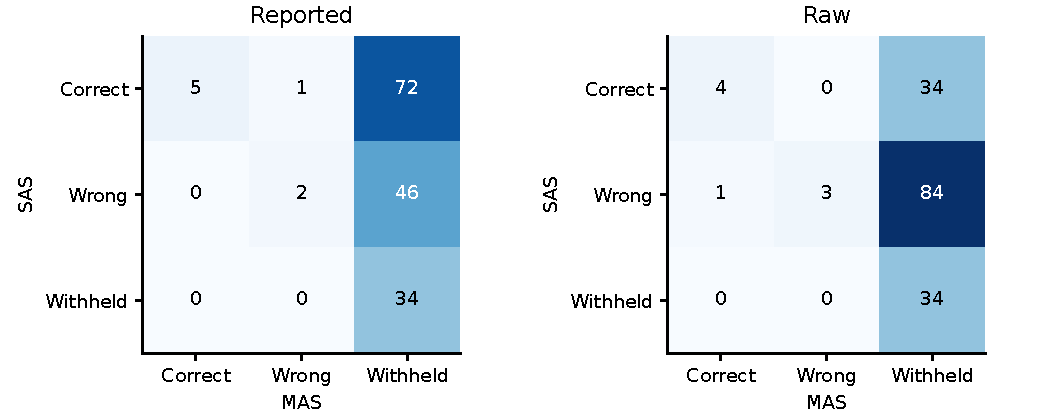
\includegraphics[width=.94\textwidth]{figures/restored_transitions.pdf}
\caption{Every primary question in the paired C/W/H transition tables. The numerical score changes which deliveries count as correct but never changes delivery itself. These are observations on the same 160 questions, not separate cohorts.}\label{fig:transitions-restored}
\end{figure}
Under reported scoring the team has no uniquely correct delivery: the paired correct gains/losses are 0/73. Under raw scoring the gains/losses are 1/34. Therefore the unqualified old statement that MAS never succeeds where SAS fails was too broad. Reported wrong gains/losses are 1/46; raw wrong gains/losses 0/85. Withholding gains/losses are 118/0 under both metrics. The reported transition table decomposes its Bowker statistic as $1+72+46=119$; the raw table gives $1+34+84=119$. The dominant movement is delivery to withholding, not correction.

Primary reported precision among delivered answers is 78/126 for SAS and 5/8 for MAS. Case-IID Wilson 95\% intervals are approximately [53.2,69.9]\% and [30.6,86.3]\%, respectively; they are descriptive because selected deliveries differ and questions share reports. Primary correct-delivery Wilson intervals are [41.1,56.4]\% and [1.3,7.1]\%; wrong-delivery intervals are [23.4,37.5]\% and [0.6,5.4]\%. These cannot replace paired cluster intervals or justify equal reliability.

\newpage
\subsection{Four endpoints, weighting and influence}
\begin{longtable}{lrrrr}
\caption{Four Study A endpoints: MAS minus SAS, percentage points. Intervals use 50 report clusters; company sensitivity uses 36. The four 98.75\% marginal intervals target approximate family coverage, not an exact finite-sample guarantee.}\label{tab:primary-ci}\\
Endpoint & $\Delta$ & Report 95\% & Report 98.75\% & Company 95\%\\\toprule\endfirsthead
Endpoint & $\Delta$ & Report 95\% & Report 98.75\% & Company 95\%\\\toprule\endhead
Reported correct & -45.62 & [-53.90, -36.55] & [-56.25, -34.09] & [-53.47, -36.44]\\
Reported wrong & -28.12 & [-37.09, -20.13] & [-39.34, -18.08] & [-38.36, -19.76]\\
Raw correct & -20.62 & [-28.26, -13.37] & [-30.29, -11.76] & [-28.15, -14.07]\\
Raw wrong & -53.12 & [-61.90, -44.08] & [-64.49, -41.26] & [-61.99, -43.08]\\
\bottomrule\end{longtable}
\begin{longtable}{lrrrr}
\caption{Weighting and influence sensitivity. Equal-report weighting estimates a different target. Deletion ranges are not confidence intervals; sign-flip tests require null sign symmetry.}\\
Endpoint & Equal-report $\Delta$ & 95\% interval & Leave-one-report range & Sign-flip $p$\\\toprule\endfirsthead
Endpoint & Equal-report $\Delta$ & 95\% interval & Leave-one-report range & Sign-flip $p$\\\toprule\endhead
Reported correct & -42.48 & [-52.66, -32.31] & [-46.79, -44.23] & 1.53e-05\\
Reported wrong & -30.62 & [-40.75, -20.71] & [-29.53, -26.75] & 1.53e-05\\
Raw correct & -18.74 & [-26.17, -11.83] & [-22.15, -19.08] & 1.53e-05\\
Raw wrong & -54.37 & [-64.00, -44.50] & [-54.61, -51.92] & 1.53e-05\\
\bottomrule\end{longtable}
\begin{longtable}{lrrrrrr}
\caption{Primary supplemental cluster diagnostics. CR1 uses normal tails; score uses chi-square(1). Right/left/tied counts refer to report-level event-rate differences, not independent confirmations.}\\
Endpoint & CR1 SE pp & DEFF & CR1 $p$ & Report score $p$ & Company score $p$ & R/L/tied\\\toprule\endfirsthead
Endpoint & CR1 SE pp & DEFF & CR1 $p$ & Report score $p$ & Company score $p$ & R/L/tied\\\toprule\endhead
reported C & 4.45 & 1.28 & 1.19e-24 & 6.41e-07 & 0.000127 & 0/33/17\\
reported W & 4.40 & 1.45 & 1.71e-10 & 1.84e-06 & 3.18e-05 & 1/29/20\\
raw C & 3.80 & 1.31 & 5.83e-08 & 4.26e-05 & 0.000112 & 0/21/29\\
raw W & 4.57 & 1.34 & 2.96e-31 & 6.36e-08 & 5.81e-05 & 0/41/9\\
\bottomrule\end{longtable}
Holm-adjusted report sign-flip values for the four correct/wrong endpoints are all $6.1034\times10^{-5}$. The corresponding report score-test adjusted values are $1.92\times10^{-6}$, $3.68\times10^{-6}$, $4.26\times10^{-5}$ and $2.54\times10^{-7}$ in reported-C, reported-W, raw-C, raw-W order. These are post-hoc diagnostics under different assumptions, not multiple independent confirmations. Three sign-flip results have zero more-extreme Monte Carlo draws, and one has one; their values reflect the finite 65,536-draw resolution. Company score-test $p$-values are larger (for reported correct, approximately $1.27\times10^{-4}$). The old claim that every cluster-aware adjusted value is at most $6.1\times10^{-5}$ does not extend to company-level variants.

On reported correct delivery SAS is higher on 33 reports, ties on 17, and is lower on none; raw correct delivery has 21 reports favoring SAS and 29 ties despite one question-level MAS gain. The question-weighted and equal-report estimands differ. Leave-one-report-out ranges show observed influence, not sampling confidence. Deterministic hash-based selection and potential common-company dependence limit population interpretation.

\subsection{Candidate production, reference strata and scoring discordance}
\begin{table}[ht]\centering
\begin{tabular}{lrrrrrrr}\toprule
Arm & Executable & Correct draft & C & W & Correct rejected & Wrong rejected & Invalid\\\midrule
SAS & 150 & 84 & 78 & 48 & 6 & 18 & 10\\
MAS & 10 & 5 & 5 & 3 & 0 & 2 & 150\\\bottomrule
\end{tabular}
\caption{Primary reported-score candidate/gate accounting. Invalid includes INSUFFICIENT. A review PASS does not override invalid execution.}\label{tab:stage-account}
\end{table}

Writing $q$ for executable fraction, $p$ for correct given executable, $a$ for acceptance of correct candidates and $b$ for acceptance of wrong executable candidates gives SAS $(q,p,a,b)=(150/160,84/150,78/84,48/66)$ and MAS $(10/160,5/10,5/5,3/5)$. Thus the reviewer accepts 72.7\% and 60\% of wrong executable candidates, respectively. The equality $C/N=qpa$ is exact descriptive accounting; it does not identify which intervention would change any factor independently. In the later planner study the candidate pool changes, so this fixed-pool calculation must be repeated for each arm.

\begin{longtable}{lrrr}
\caption{Study A primary reported-score outcomes by reference program (post hoc). Step and operation-family partitions overlap one another; do not sum across partitions.}\label{tab:strata}\\
Reference stratum & $n$ & SAS C/W/H & MAS C/W/H\\\toprule\endfirsthead
Reference stratum & $n$ & SAS C/W/H & MAS C/W/H\\\toprule\endhead
1 step & 104 & 52 / 29 / 23 & 5 / 3 / 96\\
2 steps & 49 & 26 / 14 / 9 & 0 / 0 / 49\\
3+ steps & 7 & 0 / 5 / 2 & 0 / 0 / 7\\
single add/subtract & 40 & 16 / 12 / 12 & 1 / 0 / 39\\
single ratio/product & 59 & 34 / 14 / 11 & 4 / 3 / 52\\
multi-step arithmetic & 56 & 26 / 19 / 11 & 0 / 0 / 56\\
table aggregate & 5 & 2 / 3 / 0 & 0 / 0 / 5\\
\bottomrule\end{longtable}
\begin{figure}[ht]\centering
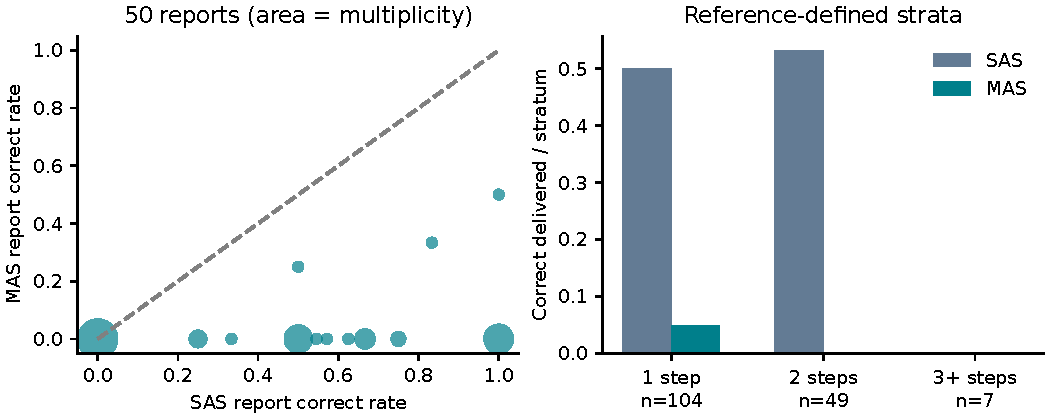
\includegraphics[width=.94\textwidth]{figures/restored_heterogeneity.pdf}
\caption{Report heterogeneity and reference-defined complexity. Repeated report-rate pairs are drawn with proportional marker area. Right: observed correct-delivery rates; stratum counts and all wrong/withheld outcomes are in Table~\ref{tab:strata}. These exploratory partitions do not isolate causal difficulty.}\label{fig:heterogeneity}
\end{figure}
There are 104 one-operation, 49 two-operation, four three-operation and three five-operation reference programs. All 56 multi-operation questions are withheld by MAS. Five questions use a table aggregate; the source-reference grammar does not directly implement max/min/sum/average. A reference operation is not necessarily the only valid solution, so grammar mismatch is a threat to comparability, not proof of impossibility.

All annotated spans are retrieved on 138 questions. SAS delivers 74 reported-correct with three invalid/insufficient programs there; MAS delivers five with 128 invalid/insufficient. In the remaining 22, SAS has four correct and MAS zero. Annotated retrieval completeness is a reference-dependent diagnostic, not proof that the question is unambiguous, that all cell identities are bound correctly, or that prompting makes the evidence usable.

Among 126 SAS deliveries, reported/raw agreement is 34 correct under both, 44 reported-only, four raw-only and 44 incorrect under both. All eight MAS deliveries agree across scores. A supported answer can therefore fail one convention while passing another. Neither convention is silently substituted for official FinQA execution scoring, and unsupported labels remain in denominators.

\subsection{Prompt, repair and resource costs}
The full paired battery below retains the direct-to-primary and primary-to-repair contrasts under both scores. SAS reported bundle gain is 28/160 with report interval [+9.76,+24.55] pp; its raw gain is 24/160 with [+8.59,+21.62]. MAS gains 5/160 with [0,+6.98]. The SAS raw wrong-delivery decrease has interval [$-17.96,+0.72$] pp: it should not be called robust merely because the case-IID exact test is near 0.05. The two prompt components are inseparable here.

Primary and repair initial candidates match on all cases. SAS repair releases one reported-correct and two wrong answers (zero raw-correct, three raw-wrong); MAS attempts 152 repairs without changing delivery. Final source-supported MAS candidates fall from ten to eight in the original trace accounting. A degenerate no-change interval does not prove equivalence in future cases.

\begin{longtable}{llrrrrr}
\caption{Timing and sampled-RSS reconciliation across original recovery and Ubuntu repeat. Summed inference excludes aborted work, model loading and restart overhead. Seconds per correct is amortized measured work, not expected retries to solve a question; undefined at zero correct.}\label{tab:resource-reconcile}\\
Run & Recipe & Hours & Median s & s/correct & Output tok & RSS GB\\\toprule\endfirsthead
Run & Recipe & Hours & Median s & s/correct & Output tok & RSS GB\\\toprule\endhead
Historical & mas-direct control & 0.821 & 17.5 & -- & 8392 & 10.901\\
Historical & mas-primary & 2.432 & 53.8 & 1751.4 & 29509 & 10.929\\
Historical & mas-repair ablation & 3.682 & 81.9 & 2651.2 & 33917 & 10.913\\
Historical & sas-direct control & 5.266 & 112.2 & 379.1 & 14449 & 10.040\\
Historical & sas-primary & 11.546 & 251.4 & 532.9 & 32657 & 10.062\\
Historical & sas-repair ablation & 13.494 & 259.9 & 614.9 & 35244 & 10.074\\
Ubuntu & mas-direct control & 0.897 & 18.5 & -- & 8392 & 10.934\\
Ubuntu & mas-primary & 3.383 & 54.6 & 2435.7 & 29509 & 10.946\\
Ubuntu & mas-repair ablation & 3.781 & 83.7 & 2722.6 & 33917 & 10.946\\
Ubuntu & sas-direct control & 5.314 & 112.7 & 382.6 & 14449 & 10.070\\
Ubuntu & sas-primary & 11.668 & 252.4 & 538.5 & 32657 & 10.075\\
Ubuntu & sas-repair ablation & 13.598 & 260.4 & 619.7 & 35244 & 10.087\\
\bottomrule\end{longtable}
\begin{longtable}{llp{.31\textwidth}rrr}
\caption{Primary stage totals in both runs. Prompt tokens count every call; they are not one context window. Stages execute sequentially while model weights remain resident.}\label{tab:stages}\\
Run & Arm & Stage & Hours & Output tok & Prompt tok\\\toprule\endfirsthead
Run & Arm & Stage & Hours & Output tok & Prompt tok\\\toprule\endhead
Hist. & MAS & extractor/select\_evidence & 0.237 & 4121 & 128047\\
Hist. & MAS & drafter/analyze\_question & 0.960 & 20441 & 134127\\
Hist. & MAS & drafter/program & 1.186 & 3507 & 390092\\
Hist. & MAS & verifier/verify\_program & 0.049 & 1440 & 94407\\
Hist. & SAS & sas/analyze\_question & 2.952 & 20479 & 134127\\
Hist. & SAS & sas/program & 6.656 & 11058 & 383588\\
Hist. & SAS & sas/verify\_program & 1.938 & 1120 & 124971\\
Ubuntu & MAS & extractor/select\_evidence & 0.346 & 4121 & 128047\\
Ubuntu & MAS & drafter/analyze\_question & 1.264 & 20441 & 134127\\
Ubuntu & MAS & drafter/program & 1.701 & 3507 & 390092\\
Ubuntu & MAS & verifier/verify\_program & 0.072 & 1440 & 94407\\
Ubuntu & SAS & sas/analyze\_question & 2.983 & 20479 & 134127\\
Ubuntu & SAS & sas/program & 6.725 & 11058 & 383588\\
Ubuntu & SAS & sas/verify\_program & 1.961 & 1120 & 124971\\
\bottomrule\end{longtable}
\begin{figure}[ht]\centering
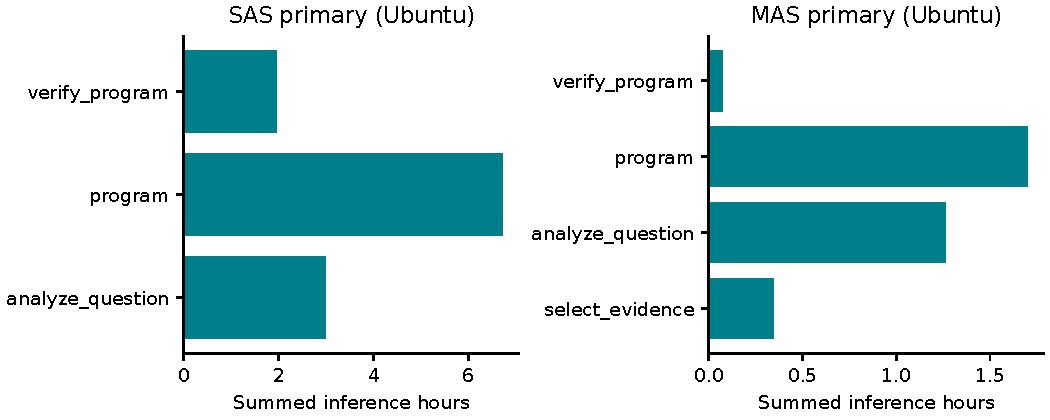
\includegraphics[width=.94\textwidth]{figures/restored_stage_work.pdf}
\caption{Stage work in the Ubuntu primary pair, summed from saved inference durations. This exposes coordination work but does not isolate a causal overhead penalty: models and prompts differ. Startup, aborted work and recovery time are excluded.}\label{fig:stage-work}
\end{figure}

Original primary medians are SAS 251.4 s and MAS 53.8 s; original amortized seconds per reported-correct answer are 532.9 and 1,751.4. Hence the historical statement of approximately 3.29 times more work per correct answer applies to that run only. Original primary prompt tokens average 4,016.8 and 4,666.7, while generated tokens average 204.1 and 184.4. The Ubuntu repeat has different durations even though scores agree. It must not inherit the original speed ratios or the original MAS repair increment of 1.25 hours. Table~\ref{tab:resource-reconcile} reports both runs distinctly.

The historical chronology is: a failed reserve check; context reduction after swap-prone probes; SAS primary swap of 44,011,520 bytes after 145 saved cases; a replay-checked continuation that later records 34,430,976 bytes of swap after seven direct-control cases; and a final continuation preserving 327 cases under kernel swap prevention. The original complete accuracy audit remains resource-invalid as an uninterrupted no-swap test. The separate Ubuntu repeat contributes zero observed swap over its saved samples, not a retroactive erasure of those failures. Its own interruptions and damaged export are disclosed in the resource section above.

\section{Conditional Mathematical Analysis and Statistical Assumptions}\label{sec:formal}
The following are established identities and conditional bounds, not novel theorems. Counts are capital $C,W,H$; rates divide by $N$. Probabilistic claims require the stated sampling assumptions and do not follow solely from deterministic trace replay.

\subsection{P1--P3: accounting, the gate bound and stage factorization}
For each case exactly one of correct delivery, wrong delivery and withholding occurs, hence $C+W+H=N$ and $\Delta C+\Delta W+\Delta H=0$. Proof: sum the exhaustive, mutually exclusive indicators. Always-withhold gives zero errors but also zero correct delivery. This identity explains why fewer wrong answers alone does not establish improvement.

For a fixed candidate set, let $A$ be the cases with correct executable candidates and $D$ the delivered cases. A gate that only accepts or rejects obeys $C_{\rm gate}=|A\cap D|\leq |A|$. Proof: an intersection is a subset of $A$. This bound assumes no rewrite, repair, new evidence or alternative candidate selection. Study A MAS has $|A|=5$, so an ideal gate over its existing drafts cannot reach SAS's 78 reported-correct deliveries. It does not rule out improved generation, representation, role allocation or a different candidate pool.

Let $E$ denote an executable candidate and $K$ numerical correctness, with delivery requiring $E$. Define $q=\Pr(E)$, $p=\Pr(K\mid E)$, $a=\Pr(D\mid E,K)$ and $b=\Pr(D\mid E,\neg K)$. Then
\begin{equation}\label{eq:stage}
 C/N=qpa,\qquad W/N=q(1-p)b,\qquad H/N=1-qpa-q(1-p)b.
\end{equation}
These empirical-frequency equalities follow from the chain rule, not independence. When a conditioning set is empty its conditional rate is undefined; the corresponding joint count remains zero. Reporting fictitious zero conditional accuracy in such a cell would be misleading.

\subsection{P4--P5: preference-sensitive utility and corrected repair break-even}\label{sec:utility}
For chosen penalties $\lambda,\kappa\geq0$, define
\begin{equation}
 U=(C-\lambda W-\kappa H)/N.
\end{equation}
The original observed primary reported-score difference is
\begin{equation}
 U_{\rm SAS}-U_{\rm MAS}=(73-45\lambda+118\kappa)/160,
\end{equation}
and the raw-score difference is $(33-85\lambda+118\kappa)/160$. Proof: substitute the observed counts. Thus switch points are $(73+118\kappa)/45$ and $(33+118\kappa)/85$, respectively. These are sample-specific preference calculations, not calibrated institutional risk thresholds or prospective optimization results.

At $\kappa=0$, reported-score MAS beats SAS only for $\lambda>73/45\approx1.622$ and beats always-withhold only for $\lambda<5/3\approx1.667$. Both constraints are necessary for MAS to be best among these three policies. With withholding cost, the MAS-versus-always-withhold condition becomes $\lambda<(5+8\kappa)/3$. The raw-score SAS/MAS switch at $\kappa=0$ is $33/85\approx0.388$; one must not transfer the narrow reported-score optimality region to raw scoring. No empirical estimate of the appropriate penalties is available.

Repair changes SAS by $(\Delta C,\Delta W,\Delta H)=(1,2,-3)$ reported and $(0,3,-3)$ raw. Consequently
\begin{equation}\label{eq:repair}
 \Delta U_{\rm rep}=(1-2\lambda+3\kappa)/160,\qquad
 \Delta U_{\rm raw}=(-3\lambda+3\kappa)/160.
\end{equation}
The old manuscript omitted $3\kappa$; its formula is correct only at zero withholding cost. Subtract an additional measured-cost term $\gamma\Delta t$ if time is priced per question. A positive time cost lowers repair utility, but does not automatically make it negative for every penalty choice. MAS's unchanged outcomes give zero outcome-utility change; additional work is unfavorable if time has positive cost. Under the prespecified correct/wrong criterion SAS repair fails regardless of a post-hoc favorable loss function.

\begin{figure}[ht]\centering
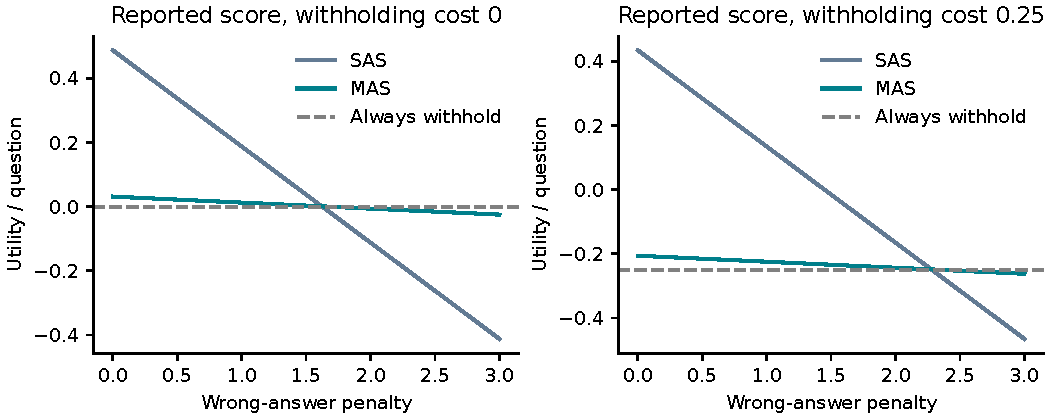
\includegraphics[width=.94\textwidth]{figures/restored_utility.pdf}
\caption{Observed reported-score utility with the always-withhold policy included. Curves are exact transformations of counts, not fitted predictions or confidence bands. Loss weights were not estimated from a financial institution.}\label{fig:utility}
\end{figure}

\subsection{P6: memory accounting with explicit residency assumptions}
If each distinct tensor $j$ has $n_j$ stored elements with effective storage $b_j$ bits per element, its storage is $n_jb_j/8$. If all such storage is actually resident simultaneously without swapping/compression, and runtime buffers occupy disjoint resident pages, a bookkeeping bound is
\begin{equation}
 M_{\rm resident}\geq\sum_j n_j b_j/8+M_{\rm KV}+M_{\rm other}.
\end{equation}
Proof: add the disjoint resident allocations, counting a truly shared tensor once. Effective bits must include block scales and other encoding overhead. File headers, padding, shared mapped pages and allocator reporting prevent treating file size as an exact RSS component. Summed process RSS may double-count shared pages; the experiments use no mmap, but this is not a universal memory-accounting theorem. Windows commit is a different measure. Table~\ref{tab:weights} explains why fewer parameters can occupy more storage at higher precision without claiming a causal precision effect on accuracy.

\subsection{P7: bounded-cluster uncertainty, with its limits}
For independent report contributions $D_g\in[-1,1]$ and fixed weights $w_g=n_g/N$, Hoeffding's inequality \citep{hoeffding} yields
\begin{equation}
 \Pr\!\left(\left|\sum_g w_g(D_g-\mathbb E D_g)\right|\geq\epsilon\right)
 \leq2\exp\!\left(-\frac{\epsilon^2}{2\sum_gw_g^2}\right),\qquad
 G_{\rm eff}=1/\sum_g w_g^2.
\end{equation}
The range of $w_gD_g$ is $2w_g$; substituting these ranges into the bounded-sum inequality proves the expression. Setting its right side to $\alpha$ gives half-width $\sqrt{2\sum_gw_g^2\log(2/\alpha)}$. Replacing $\alpha$ by $\alpha/4$ and applying the union bound gives a four-endpoint bound, assuming all four marginal conditions hold.

Observed sizes give $G_{\rm eff}=36.99$ for reports and 19.88 for companies, with 95\% half-widths 44.66 and 60.93 pp. The report four-endpoint half-width is 52.38 pp. The reported-correct $-45.625$ pp difference barely excludes zero with the report single-endpoint bound, but not with the family or company bound. This is conservative conditional uncertainty for fixed observed weights, not a design-based guarantee for deterministic report selection, a random-denominator population ratio, or dependence across companies. The effective-cluster number is weight concentration, not the literal number of independent reports.

\subsection{P8--P10: score disagreements and procedure-specific evidence bounds}
P8 follows by partitioning deliveries into both-correct, reported-only, raw-only and neither: $C_{\rm rep}-C_{\rm raw}=R_{\rm only}-E_{\rm only}$. Thus $78-38=44-4$. It does not decide which scoring convention best represents the task.

For P9, conditional exact McNemar with $n_d=b+c>0$ discordances has minimum two-sided value $\min(1,2^{1-n_d})$, attained when all discordances point one way. Proof: the smallest nonempty binomial tail under probability $1/2$ is $2^{-n_d}$; double it. Thus this procedure requires at least six discordances for $p<0.05$ and eight for $p<0.0125$. Four planner gains give $p=0.125$; five MAS prompt-bundle gains give $p=0.0625$. This is \emph{not} a claim that no other test could reject, nor evidence of no effect.

For P10, define the recorded cluster score statistic $Q=(\sum_g S_g)^2/\sum_g S_g^2$, where $S_g$ sums paired event differences and the denominator is nonzero. Cauchy--Schwarz gives $Q\leq G'$ for $G'$ nonzero cluster sums. Under the particular asymptotic $\chi^2_1$ reference, its computed tail is at least $\Pr(\chi^2_1\geq G')$. For $G'=33$ this is approximately $9.2\times10^{-9}$. The inequality bounds this statistic and reference tail only. The old claim that \emph{no valid cluster test} can provide smaller $p$-values is false: other statistics, reference distributions and assumptions have different attainable values. The archived code calls this statistic ``Durkalski''; here it is called the \emph{cluster score statistic} and its formula is supplied without claiming every variant in that literature is equivalent.

\subsection{Nonidentification and error propagation}
Across tiers, RAM, checkpoints, precision, adaptation, prompts, runtime and tasks vary together. Any observed outcomes can be matched by multiple response functions assigning different effects to RAM; the effect of changing RAM alone is unidentified without additional controlled comparisons or modeling assumptions. The same is true of a universal architecture effect. Within Study A, the bottleneck is descriptively located before delivery, but its cause can involve prompts, representation, role allocation, source suggestions or model capability.

A message-only Markov chain/data-processing account would require downstream access to evidence only through upstream messages. Here every role also sees source evidence. Correlated errors and poor verification are observed, but a Markov cascade, an information-loss rate or a causal coordination penalty is not estimated. Stage durations quantify observed work; they do not identify the counterfactual cost of removing a role while preserving capability.

\section{Statistical Derivations and Complete Numerical Battery}\label{sec:statistics-restored}
\subsection{Paired estimands and small-discordance inference (J1--J4)}
For the paired-proportion setting of \citet{mcnemar}, let $d_i=y_{Ri}-y_{Li}\in\{-1,0,1\}$ and $\widehat\Delta=N^{-1}\sum_i d_i=(b-c)/N$. Under independent case pairs,
\begin{equation}
 \operatorname{Var}(\widehat\Delta)=\{\operatorname{Var}(y_R)+\operatorname{Var}(y_L)-2\operatorname{Cov}(y_R,y_L)\}/N.
\end{equation}
Dropping the covariance by treating arms as independent changes the sampling model. Under the multinomial paired model, a plug-in variance is $\{(b+c)-(b-c)^2/N\}/N^2$. The resulting Wald interval can misbehave near boundaries; it is not the primary uncertainty interval.

Conditional on $n_d=b+c$, the null of equal event probabilities gives $b\sim\mathrm{Binomial}(n_d,1/2)$, and
\begin{equation}
 p_{\rm exact}=\min\left(1,2\sum_{k=0}^{\min(b,c)}{n_d\choose k}2^{-n_d}\right).
\end{equation}
This exactness is conditional on independent/exchangeable pairs under the binomial model; it does not survive arbitrary within-report dependence. The asymptotic statistic is $(b-c)^2/n_d$; the implementation's corrected version is $\max(|b-c|-1,0)^2/n_d$. Both use $\chi^2_1$ approximations. The maximum with zero is required to match the code when $b=c$. At zero discordance we conventionally report $p=1$ with undefined chi-square statistics, not equivalence.

Exact conditional tests can be conservative \citep{fagerland}. Retaining them alongside bootstrap intervals exposes sparse data rather than choosing the favorable procedure. With five gains and no losses among 160 cases the Wald interval excludes zero but exact $p=0.0625$; with four gains among 96, the percentile bootstrap can also exclude zero. Neither discrepancy licenses a confident population improvement. There is no post-hoc observed-power calculation.

\subsection{Transition tables, clustering and bootstrap (J5--J7)}
For states C/W/H and paired counts $n_{ij}$, Bowker symmetry uses $Q_B=\sum_{i<j}(n_{ij}-n_{ji})^2/(n_{ij}+n_{ji})$, omitting empty pairs. Its asymptotic df is the number of nonempty pairs. Stuart--Maxwell tests marginal homogeneity with $\delta_i=n_{i\cdot}-n_{\cdot i}$, $V_{ii}=n_{i\cdot}+n_{\cdot i}-2n_{ii}$ and $V_{ij}=-(n_{ij}+n_{ji})$. Dropping a redundant category gives $Q_{SM}=\delta^\top V^+\delta$, rank df, and undefined statistics at rank zero. These are case-IID, large-sample diagnostics; sparse off-diagonal cells and shared reports limit their tail probabilities even when the numerical statistics are reproduced exactly.

For independent clusters with sums $S_g=\sum_{i\in g}d_i$ and fixed sizes, $\operatorname{Var}(\widehat\Delta)=N^{-2}\sum_g\operatorname{Var}(S_g)$. The recorded CR1 estimate is
\begin{equation}
 \widehat V_{CR1}=\frac{G}{G-1}\frac{1}{N^2}\sum_g(S_g-\widehat\Delta n_g)^2.
\end{equation}
Its normal-tail $z$ test is asymptotic; the $G/(G-1)$ factor does not guarantee small-sample validity. Cluster-robust methods allow within-cluster dependence under appropriate independent-cluster regularity conditions \citep{cameron}. The score statistic of P10 instead uses uncentered squared cluster sums under its zero-mean null. It reduces to the uncorrected McNemar statistic for singleton clusters. Neither procedure is universally finite-sample valid.

The empirical variance ratio $\widehat V_{CR1}/\widehat V_{IID}$ is a descriptive design effect, not proof that one study has exactly $N/\mathrm{DEFF}$ independent observations. The earlier draft also inferred an intraclass correlation from a common-correlation approximation; heterogeneous binary paired differences do not identify such an ICC. We retain the computed design effects, but exclude that unsupported interpretation.

Cluster bootstrap draws $G$ whole reports with replacement, retaining all paired questions, and recomputes $\sum_g S_g^*/\sum_g n_g^*$. It targets a question-weighted ratio under exchangeable independent report sampling with finite moments and nonzero denominator. Equal-report averaging instead estimates $G^{-1}\sum_g S_g/n_g$. Neither is automatically appropriate to every target population. The 10,000-draw NumPy seed-42 implementation uses linear percentiles; source audit Python-indexed quantiles are kept separately. Percentile intervals are approximate and may under-cover with few discordant clusters. If all observed changes have one sign, the bootstrap cannot synthesize unseen opposite changes; it need not touch zero. This corrects the old blanket statement that such intervals always do so.

\subsection{Sign procedures, multiplicity and interpretation (J8--J12)}
Under independent cluster sums symmetric about zero, conditioning on magnitudes makes the signs exchangeable. Enumerating all sign assignments yields an exact conditional sign-flip test; the recorded implementation enumerates at most 18 nonzero clusters and otherwise uses 65,536 random assignments with $(E+1)/(R+1)$, not zero. The report sign test instead conditions on nonzero sums and assumes independent equiprobable signs, ignoring magnitudes. Zero average effect alone implies neither null. These tests are supplemental, not randomized-treatment inference.

For valid marginal $p$-values, Holm's sorted adjustment is $\widetilde p_{(j)}=\min(1,\max_{\ell\leq j}(m-\ell+1)p_{(\ell)})$ \citep{holm}. If the first true null is rejected when $m_0$ true nulls remain, its threshold is no larger than $\alpha/m_0$; the union bound gives family error at most $\alpha$ without independent tests. This guarantee requires valid input $p$-values; it does not repair invalid cluster assumptions. The four original correct/wrong endpoints form the disclosed family; withholding is algebraically determined. Excluding its test from this family is a design choice, not a theorem forbidding testing withholding for another question.

Wilson intervals invert the independent-binomial score inequality. With $z=1.96$, their endpoints are
\begin{equation}
 \frac{\widehat p+z^2/(2n)\ \pm\ z\sqrt{\widehat p(1-\widehat p)/n+z^2/(4n^2)}}{1+z^2/n}.
\end{equation}
They remain inside [0,1] but do not account for report dependence or differing selected delivery sets. Risk differences are directly interpretable here and remain finite when discordant odds ratios separate ($b=0$ or $c=0$). This does not imply that every logistic, linear-probability or cluster-robust regression is invalid; those alternatives require their own specifications and assumptions. None is needed to reproduce these descriptive paired contrasts.

All inferential interpretations depend on a hypothetical exchangeable-case/report population, despite deterministic cohort construction and greedy decoding. There are no seed, checkpoint-family or financial-expert uncertainty estimates. Non-significance does not establish equivalence without a margin and suitable design. A small $p$-value neither makes a negative result novel nor resolves the correct/wrong/withheld trade-off. The supplemental battery is retained for transparency, not to multiply apparent evidential strength.

\subsection{All historical comparisons, both numerical scores}
The following tables reproduce all 21 saved comparisons and all 126 C/W/H endpoint rows, including raw-score 8 GB comparisons that the old PDF relegated to CSV. Values are independently recomputed after checking derived outcomes against the original raw ledgers. The complete JSON additionally retains Wald intervals, both asymptotic McNemar variants, CR1, company score tests, report sign tests and transition matrices; selected primary statistics are also printed above. Repeated arms, questions, reference scores and tests do not increase the independent sample size.

Among 28 reported C/W endpoints in the 8 GB comparison family, five case-IID exact tests are below 0.05 before adjustment; none survives Holm adjustment (minimum about 0.36). The reserved MAS critic wrong-delivery decrease 17 to 9 has unchanged reported correct count 4 to 4 but raw correct decreases 8 to 7. Thus even a favorable error comparison cannot override the both-score no-correct-loss rule. The detailed battery makes this adverse trade-off visible.

\paragraph{16 GB comparison key.}
\noindent 1. Primary: MAS vs SAS\par
\noindent 2. Direct control: MAS vs SAS\par
\noindent 3. Repair ablation: MAS vs SAS\par
\noindent 4. SAS: primary vs direct\par
\noindent 5. MAS: primary vs direct\par
\noindent 6. SAS: repair vs primary\par
\noindent 7. MAS: repair vs primary\par
\begin{longtable}{lrrrrrr}
\caption{Complete 16 GB paired endpoint battery. R: reported, X: raw; C/W/H are events. IDs are defined immediately above. All tests here are post-hoc, unadjusted sensitivity analyses; exact tests assume independent pairs, score tests independent clusters and a large-cluster approximation.}\label{tab:battery-tier16}\\
ID / score / event & L/R & gain/loss & $\Delta$ pp & Report 95\% & Exact $p$ & Score $p$\\\toprule\endfirsthead
ID / score / event & L/R & gain/loss & $\Delta$ pp & Report 95\% & Exact $p$ & Score $p$\\\toprule\endhead
1 R C & 78/5 & 0/73 & -45.62 & [-53.90, -36.55] & 2.12e-22 & 6.41e-07\\
1 R W & 48/3 & 1/46 & -28.12 & [-37.09, -20.13] & 6.82e-13 & 1.84e-06\\
1 R H & 34/152 & 118/0 & +73.75 & [+64.71, +81.93] & 6.02e-36 & 9.24e-09\\
1 X C & 38/5 & 1/34 & -20.62 & [-28.26, -13.37] & 2.1e-09 & 4.26e-05\\
1 X W & 88/3 & 0/85 & -53.12 & [-61.90, -44.08] & 5.17e-26 & 6.36e-08\\
1 X H & 34/152 & 118/0 & +73.75 & [+64.71, +81.93] & 6.02e-36 & 9.24e-09\\
2 R C & 50/0 & 0/50 & -31.25 & [-40.12, -22.63] & 1.78e-15 & 5.01e-06\\
2 R W & 66/5 & 2/63 & -38.12 & [-47.65, -29.05] & 1.16e-16 & 4.87e-07\\
2 R H & 44/155 & 112/1 & +69.38 & [+59.55, +78.77] & 2.2e-32 & 1.3e-08\\
2 X C & 14/0 & 0/14 & -8.75 & [-13.29, -4.74] & 0.000122 & 0.000465\\
2 X W & 102/5 & 2/99 & -60.62 & [-70.18, -50.63] & 4.06e-27 & 4.19e-08\\
2 X H & 44/155 & 112/1 & +69.38 & [+59.55, +78.77] & 2.2e-32 & 1.3e-08\\
3 R C & 79/5 & 0/74 & -46.25 & [-54.67, -37.06] & 1.06e-22 & 6.07e-07\\
3 R W & 50/3 & 1/48 & -29.38 & [-38.41, -21.38] & 1.78e-13 & 8.35e-07\\
3 R H & 31/152 & 121/0 & +75.62 & [+66.67, +83.87] & 7.52e-37 & 6.07e-09\\
3 X C & 38/5 & 1/34 & -20.62 & [-28.26, -13.37] & 2.1e-09 & 4.26e-05\\
3 X W & 91/3 & 0/88 & -55.00 & [-63.93, -45.86] & 6.46e-27 & 3.8e-08\\
3 X H & 31/152 & 121/0 & +75.62 & [+66.67, +83.87] & 7.52e-37 & 6.07e-09\\
4 R C & 50/78 & 32/4 & +17.50 & [+9.76, +24.55] & 1.94e-06 & 0.000465\\
4 R W & 66/48 & 9/27 & -11.25 & [-17.98, -3.90] & 0.004 & 0.007\\
4 R H & 44/34 & 4/14 & -6.25 & [-12.57, -0.64] & 0.031 & 0.050\\
4 X C & 14/38 & 27/3 & +15.00 & [+8.59, +21.62] & 8.43e-06 & 0.000402\\
4 X W & 102/88 & 15/29 & -8.75 & [-17.96, +0.72] & 0.049 & 0.080\\
4 X H & 44/34 & 4/14 & -6.25 & [-12.57, -0.64] & 0.031 & 0.050\\
5 R C & 0/5 & 5/0 & +3.12 & [+0.00, +6.98] & 0.062 & 0.096\\
5 R W & 5/3 & 3/5 & -1.25 & [-5.26, +2.55] & 0.727 & 0.527\\
5 R H & 155/152 & 5/8 & -1.88 & [-7.24, +3.43] & 0.581 & 0.491\\
5 X C & 0/5 & 5/0 & +3.12 & [+0.00, +6.98] & 0.062 & 0.096\\
5 X W & 5/3 & 3/5 & -1.25 & [-5.26, +2.55] & 0.727 & 0.527\\
5 X H & 155/152 & 5/8 & -1.88 & [-7.24, +3.43] & 0.581 & 0.491\\
6 R C & 78/79 & 1/0 & +0.62 & [+0.00, +2.04] & 1.000 & 0.317\\
6 R W & 48/50 & 2/0 & +1.25 & [+0.00, +3.40] & 0.500 & 0.157\\
6 R H & 34/31 & 0/3 & -1.88 & [-4.35, +0.00] & 0.250 & 0.083\\
6 X C & 38/38 & 0/0 & +0.00 & [+0.00, +0.00] & 1.000 & 1.000\\
6 X W & 88/91 & 3/0 & +1.88 & [+0.00, +4.35] & 0.250 & 0.083\\
6 X H & 34/31 & 0/3 & -1.88 & [-4.35, +0.00] & 0.250 & 0.083\\
7 R C & 5/5 & 0/0 & +0.00 & [+0.00, +0.00] & 1.000 & 1.000\\
7 R W & 3/3 & 0/0 & +0.00 & [+0.00, +0.00] & 1.000 & 1.000\\
7 R H & 152/152 & 0/0 & +0.00 & [+0.00, +0.00] & 1.000 & 1.000\\
7 X C & 5/5 & 0/0 & +0.00 & [+0.00, +0.00] & 1.000 & 1.000\\
7 X W & 3/3 & 0/0 & +0.00 & [+0.00, +0.00] & 1.000 & 1.000\\
7 X H & 152/152 & 0/0 & +0.00 & [+0.00, +0.00] & 1.000 & 1.000\\
\bottomrule\end{longtable}
\begin{longtable}{lrrrrrr}
\caption{16 GB full-transition diagnostics. Asymptotic case-IID assumptions may fail, especially with sparse off-diagonal cells. Rank-zero statistics are undefined, not evidence of equivalence.}\\
ID / score & Bowker Q & df & $p$ & SM Q & rank & $p$\\\toprule\endfirsthead
ID / score & Bowker Q & df & $p$ & SM Q & rank & $p$\\\toprule\endhead
1 reported & 119.00 & 3 & 1.27e-25 & 118.034 & 2 & 2.34e-26\\
1 raw & 119.00 & 3 & 1.27e-25 & 118.040 & 2 & 2.33e-26\\
2 reported & 110.06 & 3 & 1.06e-23 & 109.157 & 2 & 1.98e-24\\
2 raw & 110.04 & 3 & 1.08e-23 & 109.156 & 2 & 1.98e-24\\
3 reported & 122.00 & 3 & 2.86e-26 & 121.033 & 2 & 5.22e-27\\
3 raw & 122.00 & 3 & 2.86e-26 & 121.039 & 2 & 5.21e-27\\
4 reported & 25.15 & 3 & 1.44e-05 & 22.349 & 2 & 1.4e-05\\
4 raw & 23.29 & 3 & 3.52e-05 & 23.149 & 2 & 9.4e-06\\
5 reported & 5.50 & 2 & 0.064 & 5.500 & 2 & 0.064\\
5 raw & 5.50 & 2 & 0.064 & 5.500 & 2 & 0.064\\
6 reported & 3.00 & 2 & 0.223 & 3.000 & 2 & 0.223\\
6 raw & 3.00 & 1 & 0.083 & 3.000 & 1 & 0.083\\
7 reported & 0.00 & 0 & 1.000 & -- & 0 & 1.000\\
7 raw & 0.00 & 0 & 1.000 & -- & 0 & 1.000\\
\bottomrule\end{longtable}
\paragraph{Earlier 8 GB FinQA comparison key.}
\noindent 1. Selection52: baseline MAS vs SAS\par
\noindent 2. Selection52: control MAS vs SAS\par
\noindent 3. Selection52: crossed MAS vs SAS\par
\noindent 4. Reserved49: control MAS vs SAS\par
\noindent 5. Reserved49: crossed MAS vs SAS\par
\noindent 6. Selection52: crossed vs control MAS\par
\noindent 7. Selection52: crossed vs original-critic MAS\par
\noindent 8. Reserved49: crossed vs control MAS\par
\noindent 9. Selection52: crossed vs control SAS\par
\noindent 10. Selection52: crossed vs control SAS (analysis128+demos)\par
\noindent 11. Reserved49: crossed vs control SAS\par
\noindent 12. Selection52: baseline SAS, analysis128+demos vs direct\par
\noindent 13. Selection52: control SAS, analysis128+demos vs direct\par
\noindent 14. Selection52: crossed SAS, analysis128+demos vs direct\par
\begin{longtable}{lrrrrrr}
\caption{Complete 8 GB paired endpoint battery. R: reported, X: raw; C/W/H are events. IDs are defined immediately above. All tests here are post-hoc, unadjusted sensitivity analyses; exact tests assume independent pairs, score tests independent clusters and a large-cluster approximation.}\label{tab:battery-tier8}\\
ID / score / event & L/R & gain/loss & $\Delta$ pp & Report 95\% & Exact $p$ & Score $p$\\\toprule\endfirsthead
ID / score / event & L/R & gain/loss & $\Delta$ pp & Report 95\% & Exact $p$ & Score $p$\\\toprule\endhead
1 R C & 8/2 & 0/6 & -11.54 & [-23.26, -2.00] & 0.031 & 0.083\\
1 R W & 25/19 & 8/14 & -11.54 & [-32.56, +7.69] & 0.286 & 0.257\\
1 R H & 19/31 & 18/6 & +23.08 & [+0.00, +44.44] & 0.023 & 0.064\\
1 X C & 10/3 & 0/7 & -13.46 & [-24.53, -3.85] & 0.016 & 0.052\\
1 X W & 23/18 & 9/14 & -9.62 & [-29.17, +8.33] & 0.405 & 0.297\\
1 X H & 19/31 & 18/6 & +23.08 & [+0.00, +44.44] & 0.023 & 0.064\\
2 R C & 8/3 & 0/5 & -9.62 & [-18.33, -2.00] & 0.062 & 0.059\\
2 R W & 23/19 & 4/8 & -7.69 & [-21.82, +9.30] & 0.388 & 0.371\\
2 R H & 21/30 & 12/3 & +17.31 & [-2.08, +34.29] & 0.035 & 0.117\\
2 X C & 10/5 & 0/5 & -9.62 & [-18.33, -2.00] & 0.062 & 0.059\\
2 X W & 21/17 & 4/8 & -7.69 & [-21.82, +9.30] & 0.388 & 0.371\\
2 X H & 21/30 & 12/3 & +17.31 & [-2.08, +34.29] & 0.035 & 0.117\\
3 R C & 10/3 & 0/7 & -13.46 & [-28.85, -2.00] & 0.016 & 0.108\\
3 R W & 16/15 & 6/7 & -1.92 & [-15.69, +15.26] & 1.000 & 0.808\\
3 R H & 26/34 & 13/5 & +15.38 & [-6.98, +34.43] & 0.096 & 0.194\\
3 X C & 12/5 & 0/7 & -13.46 & [-28.85, -2.00] & 0.016 & 0.108\\
3 X W & 14/13 & 6/7 & -1.92 & [-15.69, +15.26] & 1.000 & 0.808\\
3 X H & 26/34 & 13/5 & +15.38 & [-6.98, +34.43] & 0.096 & 0.194\\
4 R C & 8/4 & 1/5 & -8.16 & [-16.22, +0.00] & 0.219 & 0.102\\
4 R W & 20/17 & 6/9 & -6.12 & [-27.27, +10.91] & 0.607 & 0.513\\
4 R H & 21/28 & 12/5 & +14.29 & [+1.72, +31.71] & 0.143 & 0.052\\
4 X C & 14/8 & 1/7 & -12.24 & [-20.00, -4.35] & 0.070 & 0.034\\
4 X W & 14/13 & 6/7 & -2.04 & [-22.50, +13.73] & 1.000 & 0.819\\
4 X H & 21/28 & 12/5 & +14.29 & [+1.72, +31.71] & 0.143 & 0.052\\
5 R C & 9/4 & 1/6 & -10.20 & [-20.83, +0.00] & 0.125 & 0.132\\
5 R W & 20/9 & 3/14 & -22.45 & [-38.71, -7.50] & 0.013 & 0.022\\
5 R H & 20/36 & 19/3 & +32.65 & [+17.39, +46.88] & 0.000855 & 0.009\\
5 X C & 15/7 & 1/9 & -16.33 & [-26.15, -5.00] & 0.021 & 0.046\\
5 X W & 14/6 & 3/11 & -16.33 & [-31.43, -3.77] & 0.057 & 0.033\\
5 X H & 20/36 & 19/3 & +32.65 & [+17.39, +46.88] & 0.000855 & 0.009\\
6 R C & 3/3 & 0/0 & +0.00 & [+0.00, +0.00] & 1.000 & 1.000\\
6 R W & 19/15 & 1/5 & -7.69 & [-17.74, +2.08] & 0.219 & 0.157\\
6 R H & 30/34 & 5/1 & +7.69 & [-2.08, +17.74] & 0.219 & 0.157\\
6 X C & 5/5 & 0/0 & +0.00 & [+0.00, +0.00] & 1.000 & 1.000\\
6 X W & 17/13 & 1/5 & -7.69 & [-17.74, +2.08] & 0.219 & 0.157\\
6 X H & 30/34 & 5/1 & +7.69 & [-2.08, +17.74] & 0.219 & 0.157\\
7 R C & 4/3 & 0/1 & -1.92 & [-5.77, +0.00] & 1.000 & 0.317\\
7 R W & 22/15 & 3/10 & -13.46 & [-25.00, -1.85] & 0.092 & 0.052\\
7 R H & 26/34 & 11/3 & +15.38 & [+2.13, +27.66] & 0.057 & 0.046\\
7 X C & 6/5 & 0/1 & -1.92 & [-5.77, +0.00] & 1.000 & 0.317\\
7 X W & 20/13 & 3/10 & -13.46 & [-25.00, -1.85] & 0.092 & 0.052\\
7 X H & 26/34 & 11/3 & +15.38 & [+2.13, +27.66] & 0.057 & 0.046\\
8 R C & 4/4 & 0/0 & +0.00 & [+0.00, +0.00] & 1.000 & 1.000\\
8 R W & 17/9 & 2/10 & -16.33 & [-26.23, -4.26] & 0.039 & 0.046\\
8 R H & 28/36 & 10/2 & +16.33 & [+4.26, +26.23] & 0.039 & 0.046\\
8 X C & 8/7 & 1/2 & -2.04 & [-5.88, +0.00] & 1.000 & 0.317\\
8 X W & 13/6 & 1/8 & -14.29 & [-25.49, -2.17] & 0.039 & 0.071\\
8 X H & 28/36 & 10/2 & +16.33 & [+4.26, +26.23] & 0.039 & 0.046\\
9 R C & 8/10 & 2/0 & +3.85 & [+0.00, +11.54] & 0.500 & 0.317\\
9 R W & 23/16 & 4/11 & -13.46 & [-26.79, +0.00] & 0.118 & 0.108\\
9 R H & 21/26 & 9/4 & +9.62 & [-3.51, +23.21] & 0.267 & 0.197\\
9 X C & 10/12 & 2/0 & +3.85 & [+0.00, +11.54] & 0.500 & 0.317\\
9 X W & 21/14 & 4/11 & -13.46 & [-26.79, +0.00] & 0.118 & 0.108\\
9 X H & 21/26 & 9/4 & +9.62 & [-3.51, +23.21] & 0.267 & 0.197\\
10 R C & 9/9 & 1/1 & +0.00 & [+0.00, +0.00] & 1.000 & 1.000\\
10 R W & 20/10 & 3/13 & -19.23 & [-38.03, -2.08] & 0.021 & 0.068\\
10 R H & 23/33 & 13/3 & +19.23 & [+2.08, +38.03] & 0.021 & 0.068\\
10 X C & 11/10 & 1/2 & -1.92 & [-6.25, +0.00] & 1.000 & 0.317\\
10 X W & 18/9 & 3/12 & -17.31 & [-34.78, -1.85] & 0.035 & 0.072\\
10 X H & 23/33 & 13/3 & +19.23 & [+2.08, +38.03] & 0.021 & 0.068\\
11 R C & 8/9 & 1/0 & +2.04 & [+0.00, +5.56] & 1.000 & 0.317\\
11 R W & 20/20 & 3/3 & +0.00 & [-10.64, +8.62] & 1.000 & 1.000\\
11 R H & 21/20 & 3/4 & -2.04 & [-12.28, +10.42] & 1.000 & 0.739\\
11 X C & 14/15 & 1/0 & +2.04 & [+0.00, +5.56] & 1.000 & 0.317\\
11 X W & 14/14 & 3/3 & +0.00 & [-10.64, +8.62] & 1.000 & 1.000\\
11 X H & 21/20 & 3/4 & -2.04 & [-12.28, +10.42] & 1.000 & 0.739\\
12 R C & 8/9 & 2/1 & +1.92 & [-4.26, +8.77] & 1.000 & 0.564\\
12 R W & 25/24 & 5/6 & -1.92 & [-12.07, +12.50] & 1.000 & 0.763\\
12 R H & 19/19 & 6/6 & +0.00 & [-15.22, +11.27] & 1.000 & 1.000\\
12 X C & 10/10 & 2/2 & +0.00 & [-7.41, +7.69] & 1.000 & 1.000\\
12 X W & 23/23 & 5/5 & +0.00 & [-10.00, +13.95] & 1.000 & 1.000\\
12 X H & 19/19 & 6/6 & +0.00 & [-15.22, +11.27] & 1.000 & 1.000\\
13 R C & 8/9 & 2/1 & +1.92 & [-5.41, +10.53] & 1.000 & 0.655\\
13 R W & 23/20 & 4/7 & -5.77 & [-18.75, +6.82] & 0.549 & 0.405\\
13 R H & 21/23 & 6/4 & +3.85 & [-7.55, +15.91] & 0.754 & 0.527\\
13 X C & 10/11 & 2/1 & +1.92 & [-5.41, +10.53] & 1.000 & 0.655\\
13 X W & 21/18 & 4/7 & -5.77 & [-18.75, +6.82] & 0.549 & 0.405\\
13 X H & 21/23 & 6/4 & +3.85 & [-7.55, +15.91] & 0.754 & 0.527\\
14 R C & 10/9 & 0/1 & -1.92 & [-6.25, +0.00] & 1.000 & 0.317\\
14 R W & 16/10 & 2/8 & -11.54 & [-27.27, +0.00] & 0.109 & 0.134\\
14 R H & 26/33 & 8/1 & +13.46 & [+2.17, +28.26] & 0.039 & 0.071\\
14 X C & 12/10 & 0/2 & -3.85 & [-9.26, +0.00] & 0.500 & 0.157\\
14 X W & 14/9 & 2/7 & -9.62 & [-22.73, +0.00] & 0.180 & 0.132\\
14 X H & 26/33 & 8/1 & +13.46 & [+2.17, +28.26] & 0.039 & 0.071\\
\bottomrule\end{longtable}
\begin{longtable}{lrrrrrr}
\caption{8 GB full-transition diagnostics. Asymptotic case-IID assumptions may fail, especially with sparse off-diagonal cells. Rank-zero statistics are undefined, not evidence of equivalence.}\\
ID / score & Bowker Q & df & $p$ & SM Q & rank & $p$\\\toprule\endfirsthead
ID / score & Bowker Q & df & $p$ & SM Q & rank & $p$\\\toprule\endhead
1 reported & 9.20 & 3 & 0.027 & 9.000 & 2 & 0.011\\
1 raw & 10.20 & 3 & 0.017 & 9.947 & 2 & 0.007\\
2 reported & 7.27 & 3 & 0.064 & 7.119 & 2 & 0.028\\
2 raw & 7.27 & 3 & 0.064 & 7.119 & 2 & 0.028\\
3 reported & 7.33 & 3 & 0.062 & 7.311 & 2 & 0.026\\
3 raw & 7.33 & 3 & 0.062 & 7.311 & 2 & 0.026\\
4 reported & 4.92 & 3 & 0.178 & 3.977 & 2 & 0.137\\
4 raw & 5.48 & 3 & 0.140 & 5.000 & 2 & 0.082\\
5 reported & 12.67 & 3 & 0.005 & 11.712 & 2 & 0.003\\
5 raw & 12.68 & 3 & 0.005 & 11.971 & 2 & 0.003\\
6 reported & 2.67 & 1 & 0.102 & 2.667 & 1 & 0.102\\
6 raw & 2.67 & 1 & 0.102 & 2.667 & 1 & 0.102\\
7 reported & 4.77 & 2 & 0.092 & 4.769 & 2 & 0.092\\
7 raw & 4.77 & 2 & 0.092 & 4.769 & 2 & 0.092\\
8 reported & 5.33 & 1 & 0.021 & 5.333 & 1 & 0.021\\
8 raw & 5.78 & 2 & 0.056 & 5.778 & 2 & 0.056\\
9 reported & 3.92 & 2 & 0.141 & 3.923 & 2 & 0.141\\
9 raw & 3.92 & 2 & 0.141 & 3.923 & 2 & 0.141\\
10 reported & 7.40 & 3 & 0.060 & 6.452 & 2 & 0.040\\
10 raw & 7.57 & 3 & 0.056 & 6.273 & 2 & 0.043\\
11 reported & 1.00 & 2 & 0.607 & 1.000 & 2 & 0.607\\
11 raw & 1.00 & 2 & 0.607 & 1.000 & 2 & 0.607\\
12 reported & 1.00 & 3 & 0.801 & 0.375 & 2 & 0.829\\
12 raw & 1.44 & 3 & 0.695 & 0 & 2 & 1.000\\
13 reported & 3.11 & 3 & 0.375 & 0.897 & 2 & 0.639\\
13 raw & 3.11 & 3 & 0.375 & 0.897 & 2 & 0.639\\
14 reported & 6.44 & 2 & 0.040 & 6.444 & 2 & 0.040\\
14 raw & 6.50 & 3 & 0.090 & 6.235 & 2 & 0.044\\
\bottomrule\end{longtable}

\section{Worked Examples and Measurement Failures}\label{sec:examples}
These examples are purposively selected illustrations, not a frequency estimate. The four original financial cases and the synthetic credit case are restored, plus a score-disagreement example. Programs below are compact renderings of saved traces; they are not invented model quotations. Full recorded responses, scores, source annotations and both historical/Ubuntu records are supplied in \path{worked_example_traces.json}. Historical per-stage timing is not copied into the Ubuntu interpretation.

\subsection{Shared success: ABMD/2007/page\_52.pdf-1}
The question asks for the possible Impella purchase price including contingent payments. The reference is $56.3=11.2+45.1$ million. Catalog values A013=45.1 at text\_3 and A017=11.2 at text\_4 support both arms' one-step addition. Both executions give 56.3 and both reviewers PASS; both scoring conventions agree. The extractor selected text\_3, text\_4, text\_5 and text\_6. This case demonstrates that the team can solve some tasks, not that specialization is superior.

\subsection{Evidence found, calculation declined: AAPL/2003/page\_24.pdf-1}
The question asks for retail-segment capital expenditures before 2003, exclusive of that year's amount. The relevant sentence supplies total 290 and current-year 92, giving 198. SAS executes subtract(A005,A007), obtains 198, receives PASS and is correct under both scores. MAS selects the relevant text\_16 along with text\_17 and text\_18, but its program is
\begin{verbatim}
{"decision":"INSUFFICIENT","answer_unit":"number","steps":[]}
\end{verbatim}
The reviewer returns FAIL and the answer is withheld. Its analysis restates the requested subtraction but does not produce it. This distinguishes evidence access from candidate construction; a causal capacity floor is not identified.

\subsection{Executable does not mean meaningful: AAPL/2003/page\_24.pdf-2}
The question asks for the greatest gross-margin percentage over three years; the reference table maximum is 27.9. SAS produces eight chained subtractions, executing to 6.1 percent, and its 14B reviewer PASSes it. MAS divides A009=27 by A010=2003, executing to approximately 0.0134798, with declared percent units; its reviewer FAILs it. The saved execution value is used here rather than treating the rounded display 0.0135 as exact. A year is used as a numerical operand. Both candidates are wrong, but only SAS delivers. The grammar lacks a direct max operation; the source-member guarantee does not establish semantic suitability.

\subsection{Wrong team program accepted: PNC/2018/page\_171.pdf-1}
The question asks for home-equity lines as a percentage of total credit commitments. SAS calculates $100(16944/181612)=9.32977997$ percent and receives PASS. It matches the reported 9.3\% but not the unnormalized raw execution reference; describing it simply as correct without naming the metric would hide this distinction.

MAS computes $(31/169278)\times100/169278\approx1.08183407\times10^{-7}$ with fraction units and receives PASS. Its operands come from recorded source spans, but the calculation answers neither the reference nor a demonstrated alternative financial interpretation. It is wrong under both metrics. This is the single reported-score correct-to-wrong SAS-to-MAS transition.

\subsection{A scoring convention changes the label: ABMD/2007/page\_52.pdf-2}
SAS computes a ratio 0.5948190206 and multiplies by 100, declaring percent units. The resulting 59.48190206 matches the rounded reported label 59.5\% after unit normalization, but fails direct comparison to raw reference 0.59482. MAS emits INSUFFICIENT; although its reviewer PASSes that response, invalid execution prevents delivery. Review acceptance is therefore not itself delivery. This example illustrates both scale sensitivity and the deterministic execution guard.

\subsection{Synthetic sentinel misclassified as invention: CR-TEST-0001}
The credit packet supplies operating profit 52,852,800 PKR and debt service 13,000,000, yielding DSCR 4.0656, and current assets/liabilities 211,000,000/70,000,000, yielding 3.0143 after rounding. SAS emits valid JSON, both calculator citations and the supplied adverse-credit status. It copies the source sentinel NOT\_PROVIDED for the last-review date, citing the actual source line, while the output contract requires MISSING. The historical scorer flags this as an invented field (S6). We retain that score but do not reinterpret it as fabricated source content.

MAS's fenced outputs fail the strict JSON contract (M2), and its draft uses nonexistent calculator-style status/date spans. Its saved complete-claim-set status is false and invention field null; the 89/111 aggregate excludes it. This explains why formatting, refusal-contract and grounding errors must not be collapsed into a single factual hallucination rate. The restored examples expose limitations in the measurement as well as in the models.

\section{Restored Literature Context and Reproducibility Map}\label{sec:lit-restored}
FinMAN's financial formula/extraction/calculation decomposition and lightweight checking \citep{finman} are close antecedents. DCRC combines learned evidence auditing, program synthesis and execution \citep{dcrc}. Bench360 measures task/system trade-offs across engines, hardware and quantization choices \citep{bench360}. These motivate the recipe comparison but do not supply performance measurements for our settings. The main paper also discusses program reasoning, tool-assisted correction, selective prediction, debate, equal-budget comparisons and multiagent failure taxonomies. Positive small-agent collaboration under tool access \citep{smallagents} does not conflict with our bounded negative result. Weight quantization methods such as AWQ \citep{awq} address compression; our GGUF recipe is not an AWQ implementation. Quantized-agent process failures can change even when headline rewards remain similar \citep{quantfail}; we do not import that paper's error rates or attribute our errors to quantization alone. The study does not claim to be the first system with provenance, role specialization, executable arithmetic, repair or abstention.

Peripheral surveys of medical collaboration, cooking benchmarks, quantum-security agents and broad regulatory instruments are not restored as separate subsections: they do not validate these financial experiments. In particular, an assertion that named regulations universally require on-premises inference is not supported here. Unverified venue/version claims and external percentage gains are not copied. The coverage audit identifies these exclusions, and the original bibliography remains preserved; a shorter bibliography is not presented as an exhaustive systematic review.

The reproducibility hierarchy is: frozen raw packets and case ledgers; independent program execution/scoring; reconciliation with derived case tables; recomputed statistical tables; manuscript figures and numerical text. Hashes of original manuscripts are in \path{../preserved_versions.json}; restoration input fingerprints and checks are in \path{coverage_evidence_checks.json}. Original complete audit records and evaluator dependencies remain in \path{../../output/final_aaai/}. The handoff restore utility reconstructs the preserved evidence tree without model inference. Original unavailable SSD export/log artifacts are still unavailable; new documentation is not a substitute for those missing bytes.

\begin{verbatim}
python scripts/reporting/coverage_evidence.py --evidence PATH
python -m unittest tests.test_reporting_statistics
python -m unittest tests.test_paper_statistical_tests
\end{verbatim}

Terminology: SAS uses one model instance for potentially several stages; MAS has separate resident role instances. Q4\_K\_M names the GGUF weight quantization, not a four-bit activation or KV-cache claim. F16 names stored half-precision weights. RSS denotes resident-set accounting; Windows commit is committed virtual-memory accounting and is not a physical-RAM guarantee. Coverage is $(C+W)/N$; selective error is $W/(C+W)$ when any answers are delivered; pp denotes percentage points. Historical KYC/credit tasks test synthetic output contracts, not professional due diligence. No 32 GB measurement, general scaling curve or autonomous financial-decision validation is supplied.
